%liste des modules réalisés
%Preuve du fonctionnement de chaque modules

\subsection{Taxonomie}%Martin
\subsubsection{Approche par Word2Vec}\label{word2vecReal}
Pour tenter d'extraire la taxonomie des documents, nous avons débuté sur une approche basée sur des \textit{embeddings} construit a partir d'un Word2Vec entrainé sur un corpus français. Idéalement, ce réseau nous permettrait d'obtenir des taxonomies en comparant les mots du documents avec ceux présent dans la liste de taxonomies, et d'ajouter ceux dont la distance, définie en (~\ref{eq:distCosine}), était sous un seuil. Cette approche, ne nécessitant pas de corpus annotée semblait correspondre a nos besoins, même si il n'existait pas de cas dans la littérature scientifique ou elle fut appliquée avec succès. %Réecrire...

Après implémentation de cette méthode, plusieurs difficultés sont apparue.
D'abord, le temps d'exécution de cette méthode pour un seul document sur le texte en entier dépassait largement les limites de l'acceptable.
En effet, un document administratif est presque par nécessité très verbeux, et donc long. La majorité du texte ne nous est cependant pas utile pour notre but; 
il ne sert qu'à donner du contexte pour le lecteur et ne donne pas forcément d'information concernant le sujet du document en lui même. 

Deuxièmement, nous n'avons pas pu obtenir les résultats escomptés. Le principal obstacle venant du fait que les mots de la taxonomie peuvent être en fait des phrases, ou tout du moins de multiples mots dont les sens ne sont pas forcément corrélés.

On trouve par exemple "aménagement foncier", mais aussi "fromage au lait cru" ou bien encore "médecine physique et de réadaptation". La technique que nous utilisions pour obtenir les \textit{embeddings}, Word2Vec, ne fonctionne pas sur des \textit{groupes de mots} ou \textit{n-grammes}, mais sur des mots seuls. Doc2vec, qui lui peut fonctionner sur des n-grammes, voire des paragraphes ou documents entier a besoin d'être entrainé sur des documents qui lui apporteront le contexte nécessaire pour former des \textit{embeddings} correct.

Cependant, la taxonomie ne donne aucun contexte. Il s'agit seulement d'une liste de mot et de phrase ordonnée seulement sous la forme d'un arbre (voir figure \ref{fig:tree}). Il ne s'agit pas d'un document ordinaire, et nous pouvions pas utiliser les techniques courantes dans ce cas. 

Nous avons d'abord tenté d'améliorer la rapidité d'execution en précalculant les vecteurs de la taxonomie. Initialement, nous itérions simplement sur la liste de taxonomies, et calculions les \textit{embeddings} à la volée. En précalculant les vecteurs avant même l'execution du module d'assignement de la taxonomie nous pouvions économiser des cycles processeurs. Ensuite, plutôt que d'utiliser l'intégralité du texte, nous avons décidé de n'utiliser que les titres des arrêtés. Ainsi, nous réduisions considérablement la quantité de texte à analyser.

Pour essayer de contrer ce deuxieme problème, la décision initiale fut de transformer chaque mot de la phrase en sa racine par le procédé de la lemmatization à l'aide de la librairie spacy\cite{spacy} et d'enlever les \textit{stopwords} de la phrase.
Les \textit{stopwords} sont des mots apparent très fréquemment dans les phrases, comme les déterminants.
Ainsi la phrase "médecine physique et de réadaptation" se trouve transformée en "médecine physique réadaptation".
On utilise ensuite un Word2Vec sur chaque mot pour obtenir plusieurs vecteurs. Pour obtenir un seul vecteur que nous comparerons avec les mots du documents, nous effectuons un simple moyen-âge.

Malgré ces efforts pour contrer les problèmes rencontrés, les taxonomies
Cependant, cette solution n'as pas fonctionné et les taxonomies que nous trouvions a l'aide de ce système ne correspondait simplement pas au document analysés.

Cet échec est du a la manière dont nous utilisons les vecteurs de mots produit par Word2Vec: une comparaison simple, ne donnant qu'une metrique de similarité ne suffit pas a établir un contexte suffisant pour ajouter des taxonomies sensées. En effet, si un mot dans un titre et un mot dans la taxonomie sont identiques, alors leur métrique sera forcément faible, même si ces deux mots sont utilisés différement dans le contexte actuel. On se retrouve alors a obtenir une grande quantités de taxonomie qui ne sont pas utile. De plus, la question de la rapidité d'analyse n'as pas pu être totalement élucidée, même avec un prétraitement des vecteurs et l'utilisation des titres plutôt que du texte entier. Pour un seul document, on pouvait avoir jusqu'à plusieurs minutes de calcul. Même si l'optimisation n'était pas une priorité dans ce projet, il devenait évident que cette approche ne pouvait fonctionner.

\subsubsection{Approche par détection de mots commun}
La solution finale adaptée fut celle de simplement extraire les titres d'arrêtées administratifs, qui sont les documents a classer, et à les prétraiter par lemmatization et élimination des stopwords avant d'effectuer une simple recherche dans la taxonomie.
Si un mot de la taxonomie se trouve dans le titre de l'article administratif, alors celui ci est ajouté au document. Cette solution est non seulement bien plus simple et permet de vérifier la qualité des résultats plus aisément qu'à l'aide d'un \textit{embedding}, et elle est de plus bien plus rapide, permettant l'analyse d'un document entier en quelques secondes à peine contre plusieurs minutes à l'aide d'un Word2Vec.

\begin{figure}[h!]
  \centering
  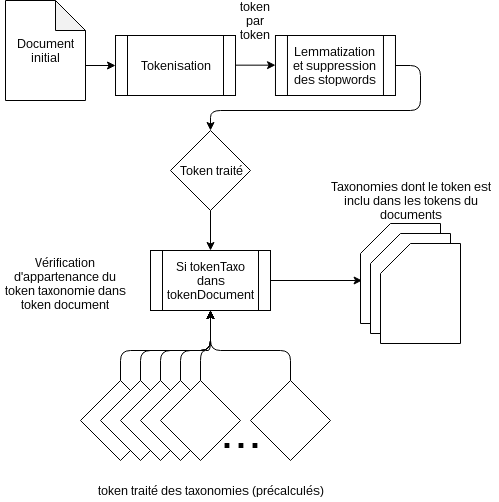
\includegraphics[width=0.7\textwidth]{diagFinalTaxo.png}
	\caption[]{Schéma fonctionnel du module d'assignement taxonomique final}
  \label{taxoFinal}
\end{figure}

\subsubsection{Parcours de l'arbre taxonomique}
\begin{figure}[h!]
  \centering
  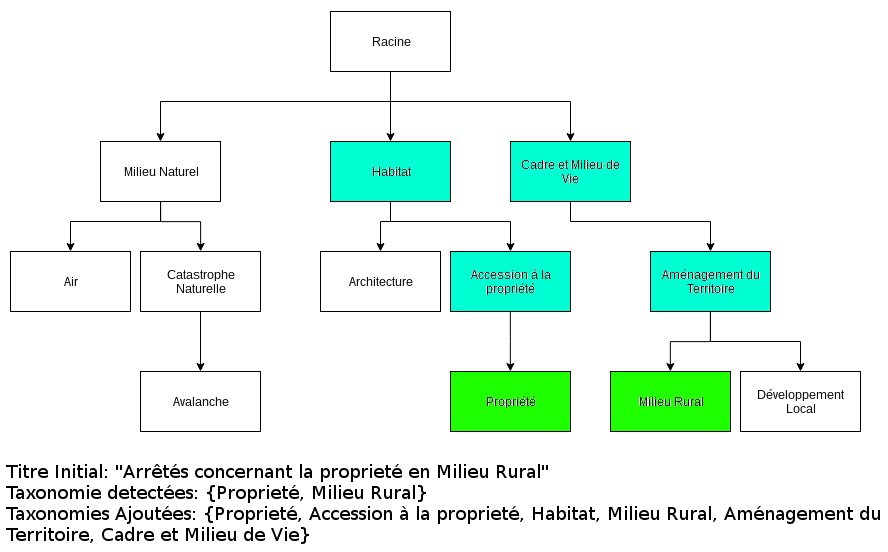
\includegraphics[width=\textwidth]{remontageArbre.png}
	\caption[]{Représentation de la technique de parcours d'arbre utilisée pour obtenir plus de taxonomies}
  \label{fig:tree}
\end{figure}


Pour obtenir une taxonomie plus vaste, nous prenons également en compte la structure de la taxonomie. En effet, celle ci se présente sous forme d'un arbre, structure que nous pouvons observer en figure~\ref{fig:tree}. Chaque sections possèdes des sous sections, qui permettent un affinage et une grande précision dans la classification.
L'idée centrale étant de considérer que si un document possède comme taxonomie une feuille ou un noeud de cette arbre, alors il doit nécessairement posséder comme taxonomie tout les parents de ce noeud. Nous remontons alors jusqu'à la racine de l'arbre depuis le noeud de la taxonomie ayant été détectée, en ajoutant à la taxonomie du document tous les noeuds que nous rencontrons en chemin. Cette approche nous permet d'obtenir une plus grande variété de taxonomie sans avoir a utiliser une analyse plus lourde sur le texte. 

\subsubsection{Classement des taxonomies}
En sortie, nous récupérons un grand nombre de taxonomie, données a la fois par la détection initiale et par le parcours d'arbre. Pour obtenir les taxonomies les plus représentative du document, nous procédons ensuite a un classement des taxonomies selon le nombre de fois ou chacune apparait dans le tableau des taxonomies. Les taxonomies qui apparaissent souvent dans le document sont donc considérées comme plus "importante" que des taxonomies apparaissant rarement.

Le parcours d'arbre apportant une très grande quantité de nouveaux mots pour chaque taxonomies, il est donc nécessaire d'équilibrer ce système. Pour se faire, nous appliquons un simple système de poids au taxonomies detectées: une taxonomie initiale aura un poids 100 supérieur a une taxonomie recupéré par le parcours d'arbre.


